\documentclass{beamer}
\usetheme{Montpellier}
\usecolortheme{beaver}
\setbeamerfont{footnote}{size=\tiny}
\setbeamerfont{footnote mark}{size=\tiny}
\setbeamerfont{cite}{size=\tiny}
%Don't use default captions, footnote errors!
%https://tex.stackexchange.com/questions/43778/aberrant-footnote-numbering-behavior-with-footnoted-captions
%\setbeamerfont{caption}{size=\scriptsize}
%\setbeamertemplate{caption}{\insertcaption}
%\setbeamercolor{caption}{fg=blue}
%\setlength\abovecaptionskip{-5pt}


%To comment out sections
\usepackage{comment}

%bibliography
\usepackage[square,sort]{natbib}
%math
\usepackage{amsmath}
%algorithm
\usepackage[boxruled,algoruled]{algorithm2e}
%caption package for better behavior
\usepackage[skip=2pt]{caption}
\captionsetup{font={color=blue,scriptsize}}
\captionsetup{labelformat=empty,labelsep=none}
\captionsetup{justification=centering}


% Define some common variables
\def\micron{$\upmu$m}
\def\deltaz{\delta_{z}} % depth resolution
\def\drn{dr_{N}} % outermost zone width
\def\rn{r_{N}} % zone plate radius
\def\NA{\mbox{N.A.}}
\def\deltaz{\delta_{z}} % depth resolution
\def\deltares{\delta_{r}} % Spatial resolution
\def\tzp{t_{\rm zp}} % Zone plate thickness
\def\tzpopt{t_{\rm zp,opt}} % Optimum thickness
\def\thetazp{\theta} % Zone plate tilt
\def\thetabragg{\theta_{\rm B}} % Bragg angle

\def\thetaellapproxu{\theta_{u}} % Rayleigh quarter wave tilt limit
\def\thetaellapproxl{\theta_{l}} % Rayleigh quarter wave tilt limit

\def\thetaellc{\theta_c} % tilt limit if coma dominates
\def\thetaella{\theta_a} % tilt limit of astigmatism dominates

\def\thetadof{\theta_{\rm DOF}} % tilt limit via depth of focus

\def\ellexactu{\ell_{u}^{\prime}}
\def\ellexactl{\ell_{l}^{\prime}}

\def\ellapproxu{\ell_{u}}
\def\ellapproxl{\ell_{l}}
\def\ellapprox0{\ell_{0}}

\def\ellapproxc{\ell_{c}}
\def\ellapproxa{\ell_{a}}

\def\ellmyers{\ell_{\rm m}}
\def\ellmyersprime{\ell_{\rm m}^{\prime}}

\def\dof{\mbox{DOF}}
\def\thetafield{\theta_{f}}
\def\npix{N_{x}}
\def\pixelsize{\Delta_{x}}
\def\pixelsizeout{\Delta_{x}^{\prime}}
\def\pixeldepth{\Delta_{z}}
\def\pixelphase{\varphi_{x}}
\def\nzpix{N_{z}}
\def\voxelfraction{\chi}
\def\pixeldepthkc{\Delta_{z,Q}}
\def\qkleincook{Q} % Klein--Cook parameter
\def\realpix{\Delta_{r}} % real space pixel size in CDI
% Define some common variables
\def\micron{$\upmu$m}
\def\deltaz{\delta_{z}} % depth resolution
\def\drn{dr_{N}} % outermost zone width
\def\rn{r_{N}} % zone plate radius
\def\NA{\mbox{N.A.}}
\def\deltaz{\delta_{z}} % depth resolution
\def\deltares{\delta_{r}} % Spatial resolution
\def\tzp{t_{\rm zp}} % Zone plate thickness
\def\tzpopt{t_{\rm zp,opt}} % Optimum thickness
\def\thetazp{\theta} % Zone plate tilt
\def\thetabragg{\theta_{\rm B}} % Bragg angle

\def\thetaellapproxu{\theta_{u}} % Rayleigh quarter wave tilt limit
\def\thetaellapproxl{\theta_{l}} % Rayleigh quarter wave tilt limit

\def\thetaellc{\theta_c} % tilt limit if coma dominates
\def\thetaella{\theta_a} % tilt limit of astigmatism dominates

\def\thetadof{\theta_{\rm DOF}} % tilt limit via depth of focus

\def\ellexactu{\ell_{u}^{\prime}}
\def\ellexactl{\ell_{l}^{\prime}}

\def\ellapproxu{\ell_{u}}
\def\ellapproxl{\ell_{l}}
\def\ellapprox0{\ell_{0}}

\def\ellapproxc{\ell_{c}}
\def\ellapproxa{\ell_{a}}

\def\ellmyers{\ell_{\rm m}}
\def\ellmyersprime{\ell_{\rm m}^{\prime}}

\def\dof{\mbox{DOF}}
\def\thetafield{\theta_{f}}
\def\npix{N_{x}}
\def\pixelsize{\Delta_{x}}
\def\pixelsizeout{\Delta_{x}^{\prime}}
\def\pixeldepth{\Delta_{z}}
\def\pixelphase{\varphi_{x}}
\def\nzpix{N_{z}}
\def\voxelfraction{\chi}
\def\pixeldepthkc{\Delta_{z,Q}}
\def\qkleincook{Q} % Klein--Cook parameter
\def\realpix{\Delta_{r}} % real space pixel size in CDI



\title{Effect of tilt on zone plate performance}
\author{Sajid Ali\inst{1} \& Chris Jacobsen\inst{2}}	
\institute[NU] 
{\inst{1}%
  Applied Physics\\
  Northwestern University\\
\inst{2}%	
	X-ray Science Divison\\
	Argonne National Lab}
\date{\today}
% If you have a file called "university-logo-filename.xxx", where xxx
% is a graphic format that can be processed by latex or pdflatex,
% resp., then you can add a logo as follows:

% \pgfdeclareimage[height=0.5cm]{university-logo}{university-logo-filename}
% \logo{\pgfuseimage{university-logo}}

% Delete this, if you do not want the table of contents to pop up at
% the beginning of each subsection:
\AtBeginSubsection[]
{
  \begin{frame}<beamer>{Outline}
    \tableofcontents[currentsection,currentsubsection]
  \end{frame}
}
\AtBeginSection[]{
	\begin{frame}
		\vfill
		\centering
		\begin{beamercolorbox}[sep=8pt,center,shadow=true,rounded=true]{title}
			\usebeamerfont{title}\insertsectionhead\par%
		\end{beamercolorbox}
		\vfill
	\end{frame}
}

% Let's get started
\begin{document}

\begin{frame}
  \titlepage
\end{frame}

\begin{frame}{Outline}
  \tableofcontents
  % You might wish to add the option [pausesections]
\end{frame}

% Section and subsections will appear in the presentation overview
% and table of contents.

\section{Introduction}

\begin{frame}{Focusing X-Rays}
	\begin{block}{}
		\begin{columns}[onlytextwidth,T]
			\column{\dimexpr\linewidth-30mm-10mm}
			\begin{itemize}
			\item Ref. index$\rightarrow$ complex,slightly $<$ 1
			\item Zone plates$\rightarrow$ monochromatic diffractive optics.
			\item Alternate rings of low/high ref. index materials placed such that the outgoing waves constructively interfere with each other at the focal spot.
			\end{itemize}
			\column{30mm}
			\begin{figure}
				\includegraphics[width=40mm]{zp}
				\caption{Illustration of zone plate \footnotemark}
			\end{figure}
		\end{columns}
	\footnotetext{\cite{jacobsen_2019}}
	\end{block}
\end{frame}


\begin{frame}{Factors affecting efficiency \& resolution}
	\begin{block}{}
		\begin{columns}[onlytextwidth,T]
			\column{\dimexpr\linewidth-30mm-10mm}
			\begin{itemize}
				\item Spatial resolution limited to finest, outermost zone width.
				\item Zones must be thick enough along beam direction to produce a phase shift of $\pi$, several um at hard x-ray energy.
			\end{itemize}
			\column{30mm}
			\begin{figure}
				\hspace*{-1.1cm}\includegraphics[width=50mm]{zp_chris}
				\caption{Thickness vs efficiency \footnotemark}
			\end{figure}
		\end{columns}
	\footnotetext{\cite{jacobsen_2019}}
	\end{block}
\end{frame}

\begin{frame}{Scalar theory is not enough}
	\begin{block}{}
		\begin{columns}[onlytextwidth,T]
			\column{\dimexpr\linewidth-30mm-10mm}
			\begin{itemize}
				\item Scalar approximation assumption $\rightarrow$ interaction between x-rays and the optic can be treated as one-step diffraction. 
				\item Klein-Cook param. : $Q_{K-C}$ indicator of 
				"diffraction regime"\footnotemark.
			\end{itemize}
			\column{30mm}
			\begin{figure}
				\hspace*{-0.75cm}\includegraphics[width=45mm]{grating}
				\caption{Volume effects in 1d gratings}
			\end{figure}
		\end{columns}
	\footnotetext{\cite{klein_ieeetsu_1967}}
	%\footnotetext{\cite{Li17}}
	\end{block}
\end{frame}


\begin{frame}{Motivation for tilt misalignment study}
	\begin{itemize}
		\item As Aspect ratios of zone plates go up\footnotemark \footnotetext{\cite{chang_natcomm_2014,parfeniukas_spie_2017,li_jvstb_2017}}, tilt misalignment needs to be understood better.
		\item Analytic limits\footnotemark \footnotetext{\cite{myers_ajp_1951,young_josa_1972}} from literature do not account for volume diffraction effects.
		\item Local bragg angle for each zone $\rightarrow$ not the focus here.
	\end{itemize}
\end{frame}


\section{Analytic limits}

\begin{frame}{Analytic limits}
	\begin{block}{}
		\begin{columns}[onlytextwidth,T]
			\column{\dimexpr\linewidth-30mm-10mm}
			\begin{itemize}
				\item Derived by using path difference between (upper) marginal, axial ray \footnotemark
					

			\end{itemize}
			\column{30mm}
			\begin{figure}
				\hspace*{-1cm}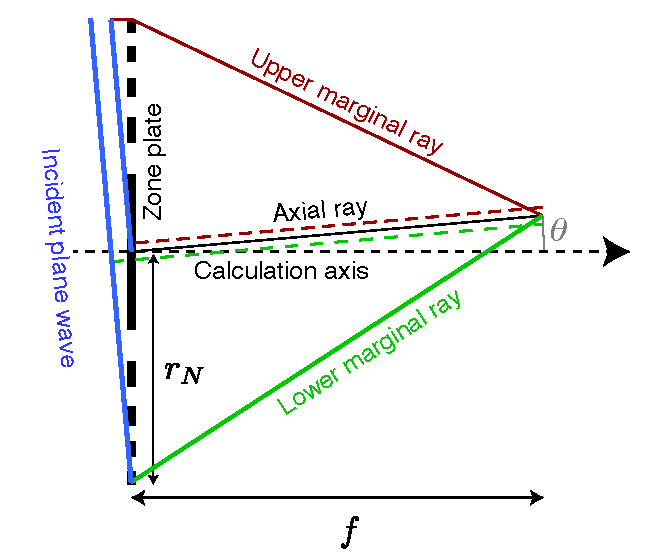
\includegraphics[width=50mm]{zp_schematic}
				\caption{Volume effects in 1d gratings}
			\end{figure}
		\end{columns}
	%\addtocounter{footnote}{-1}
	%	\footnotetext{\cite{young_josa_1972}}
	%\stepcounter{footnote}
	\footnotetext{\cite{myers_ajp_1951,young_josa_1972}}

	\end{block}
\end{frame}


\begin{frame}{Expected behavior}
	\begin{itemize}
		\item coma at soft xray, astigmatism at hard xray.
		\begin{center}
			\begin{figure}
				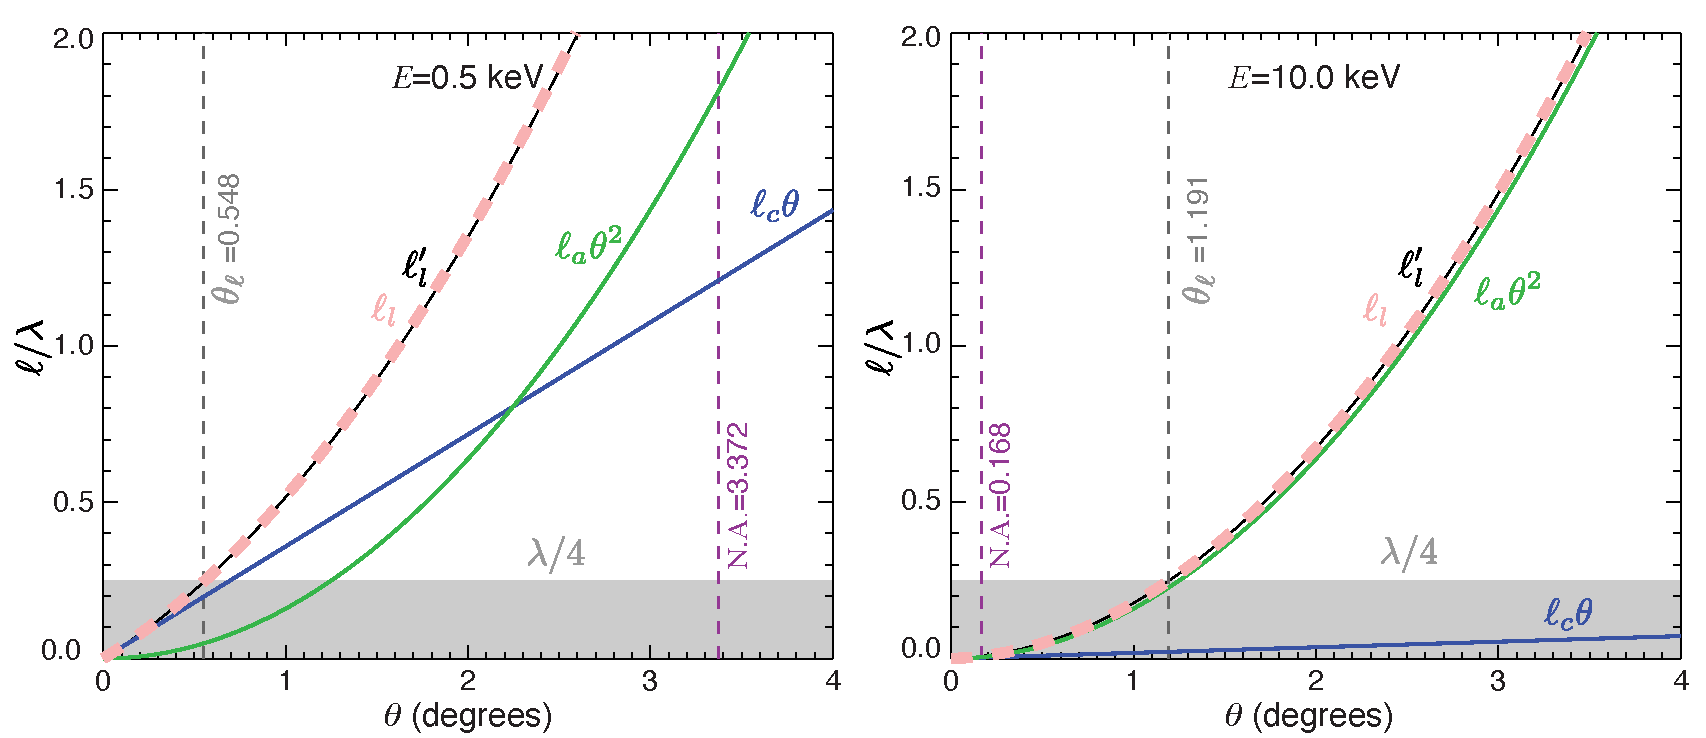
\includegraphics[scale=0.3]{path_length_terms}
				\caption{Path length terms}	
			\end{figure}
		\end{center}
	\end{itemize}
\end{frame}


\section{Implementation}
\begin{frame}{Partial Filling}
	\begin{itemize}
		\item No binary filling.
		\begin{center}
			\begin{figure}
				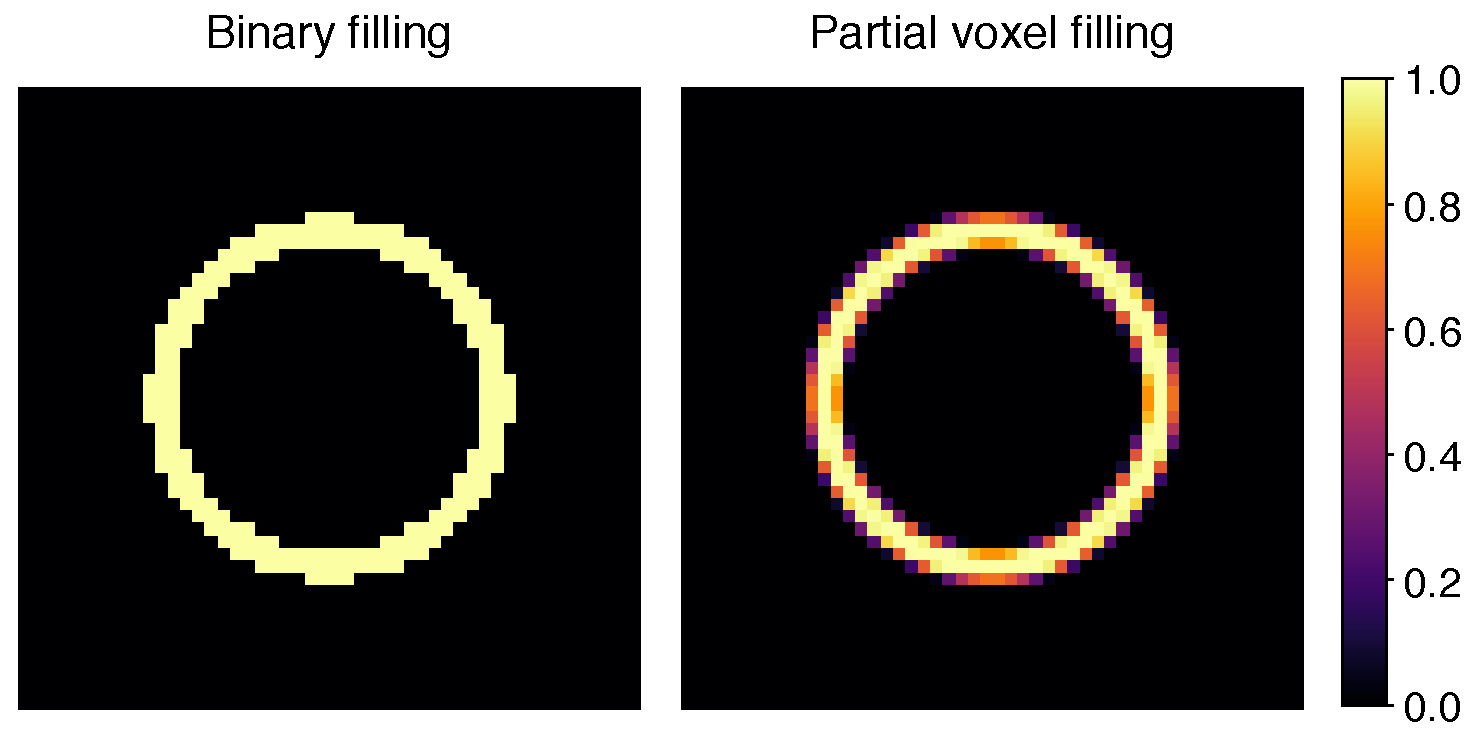
\includegraphics[scale=0.3]{partial_fill}
				\caption{Partial fil}	
			\end{figure}
		\end{center}
	\end{itemize}
\end{frame}


\begin{frame}{Multislice }
	\begin{onlyenv}<1>
		
		\begin{columns}[onlytextwidth,T]
		\column{\dimexpr\linewidth-20mm-10mm}
		\scalebox{0.65}{
			\begin{algorithm}[H] 
				% This is to hide end and get the last vertical line straight
				\SetAlgoLined\DontPrintSemicolon
				
				\SetKwFunction{SliceDiff}{SliceDiff}
				\SetKwFunction{PropShort}{PropShort}
				\SetKwFunction{PropLong}{PropLong}
				
				\tcc{initialize}
				$\psi(x,y) \xleftarrow{} 1$\;
				\tcc{diffraction within optic}
				\For{n=1,N}{ 	
					\SliceDiff{n}\;
					\PropShort{$\pixeldepth$}\;
				}
				\tcc{Propagate exit wave by a focal length $f$ to the focal plane}
				\PropLong{$f$} \;
				\caption{Optic simulation using the multislice method.}
			\end{algorithm}
		}
		\column{30mm}
			\begin{figure}
				\hspace*{-2.1cm}\includegraphics[width=60mm]{ms}
				\caption{Multi-slice schematic \footnotemark }
			\end{figure}
		\end{columns}

		\footnotetext{\cite{jacobsen_2019}}
		
		
		
	\end{onlyenv}
	
	\begin{onlyenv}<2>
		\scalebox{0.65}{
			\begin{algorithm}[H]
				%This is to hide Begin keyword
				\SetKwProg{myproc}{Procedure}{}{}
				\myproc{\SliceDiff{n}}{
					\tcc{Apply refractive effect of slice using }	
					$\psi(x,y) = \psi(x,y) \odot \exp\Bigl[i\, \frac{2\pi \pixeldepth}{\lambda} \bigl(\delta(x,y)+i\beta(x,y)\bigr)\Bigr]$ \;
					\KwRet\;}
				
				\SetKwProg{myproc}{Procedure}{}{}
				\myproc{\PropShort{$\pixeldepth$}}{
					\tcc{Free space propagation from source $s$ to destination $d$ plane}	
					$\psi_{s}(x,y) \xrightarrow{\mathcal{F}}\Psi(u,v)$\;
					$\Psi(u,v) = \Psi(u,v) \odot \exp\Bigl[-i\, \frac{2\pi \pixeldepth}{\lambda} \sqrt{1-\lambda^{2}(u^{2}+v^{2})}\Bigr]$\;
					$\Psi(u,v) \xrightarrow{\mathcal{F}^{-1}}\psi_d(x,y)$\;
					\KwRet\;}
				
				\SetKwProg{myproc}{Procedure}{}{}
				\myproc{\PropLong{$f$}}{
					\tcc{Free space propagation from source $s$ to destination $d$ plane}	
					$\psi^{\prime}(x,y) = \psi_{s}(x,y) \odot \exp\Bigl[-i\,\frac{2\pi f}{\lambda}  \sqrt{x_{s}^{2}+x_{s}^{2}+f^{2}}\Bigr]$\;
					$\psi^{\prime}(x,y) \xrightarrow{\mathcal{F}} \Psi^{\prime}(x,y)$\;
					$\Psi_{d}(x,y) = \Psi^{\prime}(x,y) \odot \exp\Bigl[-i\,\frac{2\pi f}{\lambda} \sqrt{x_{d}^{2}+x_{d}^{2}+f^{2}}\Bigr]$\;
					$\psi_{d}(x,y) = \frac{i\pixelsize^2}{\lambda f} \Psi_{d}(x,y)$\;
					\KwRet\;}
				%				\caption{Optic simulation using the multislice method.}
			\end{algorithm}
		}
	\end{onlyenv}
\end{frame}


\begin{frame}{Approaches}
	\begin{block}{}
		\begin{columns}[onlytextwidth,T]
			\column{\dimexpr\linewidth-30mm-10mm}
			\begin{itemize}
				\item Two approaches.
			\end{itemize}
			\column{30mm}
			\begin{figure}
				\hspace*{-1cm}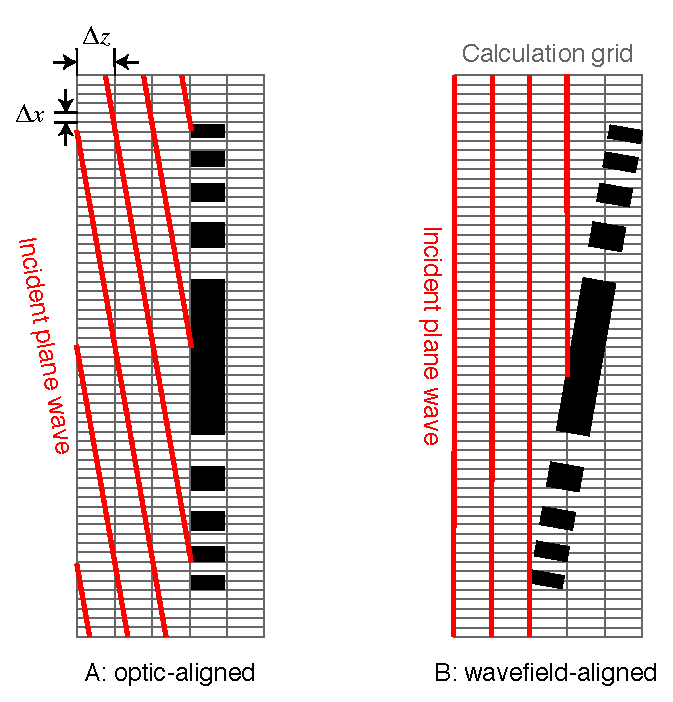
\includegraphics[width=50mm]{tilted_zp_grids}
				\caption{Approaches}
			\end{figure}
		\end{columns}
	\end{block}
\end{frame}


\section{Results}
\begin{frame}{soft x-ray}
	\begin{itemize}
		\item Coma predicted.
		\begin{center}
			\begin{figure}
				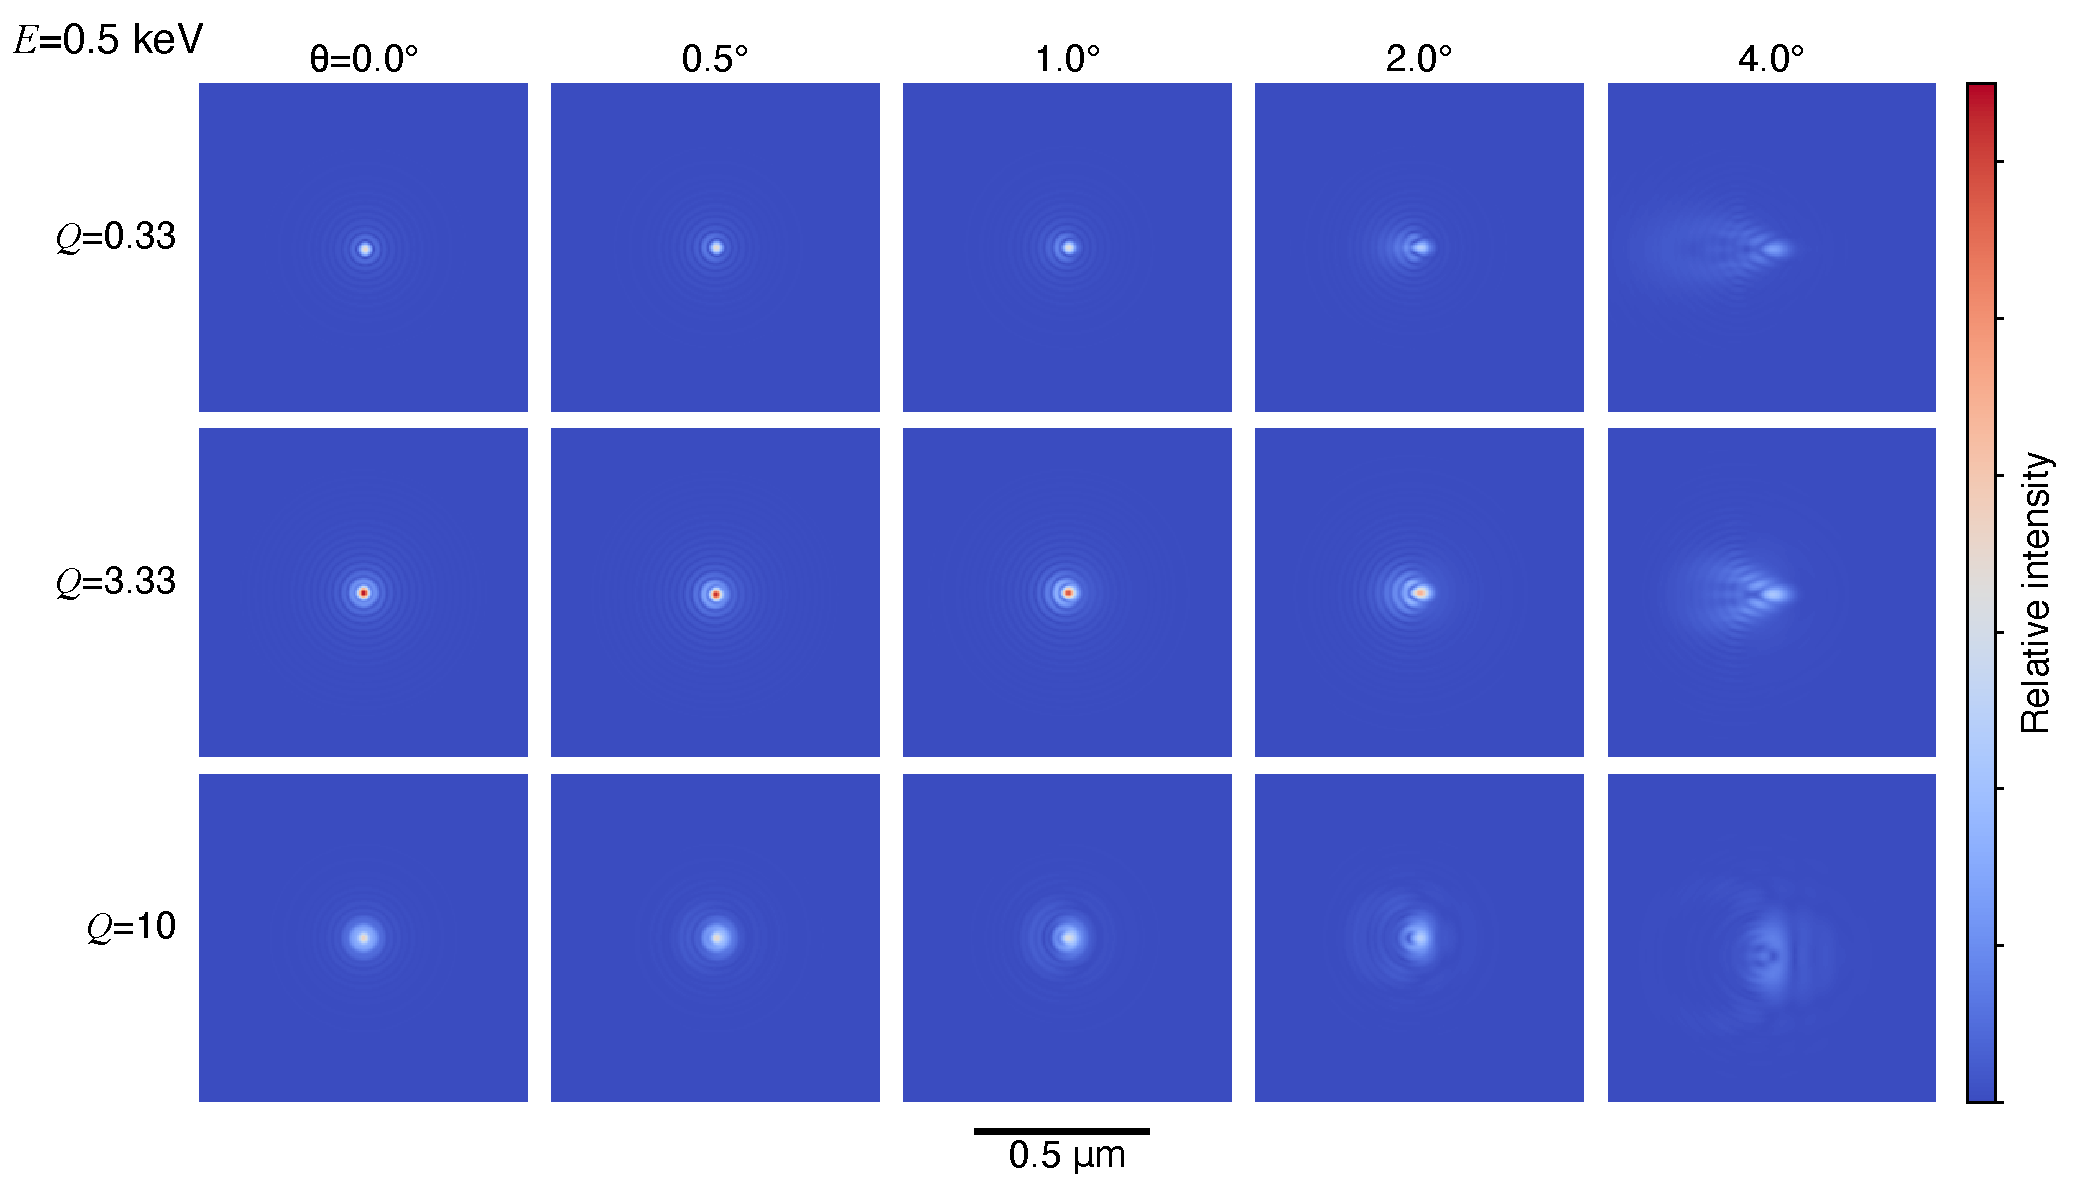
\includegraphics[scale=0.275]{foc_spot_half}
				\caption{Partial fil}	
			\end{figure}
		\end{center}
	\end{itemize}
\end{frame}

\begin{frame}{hard x-ray}
	\begin{itemize}
		\item Astigmatism predicted.
		\begin{center}
			\begin{figure}
				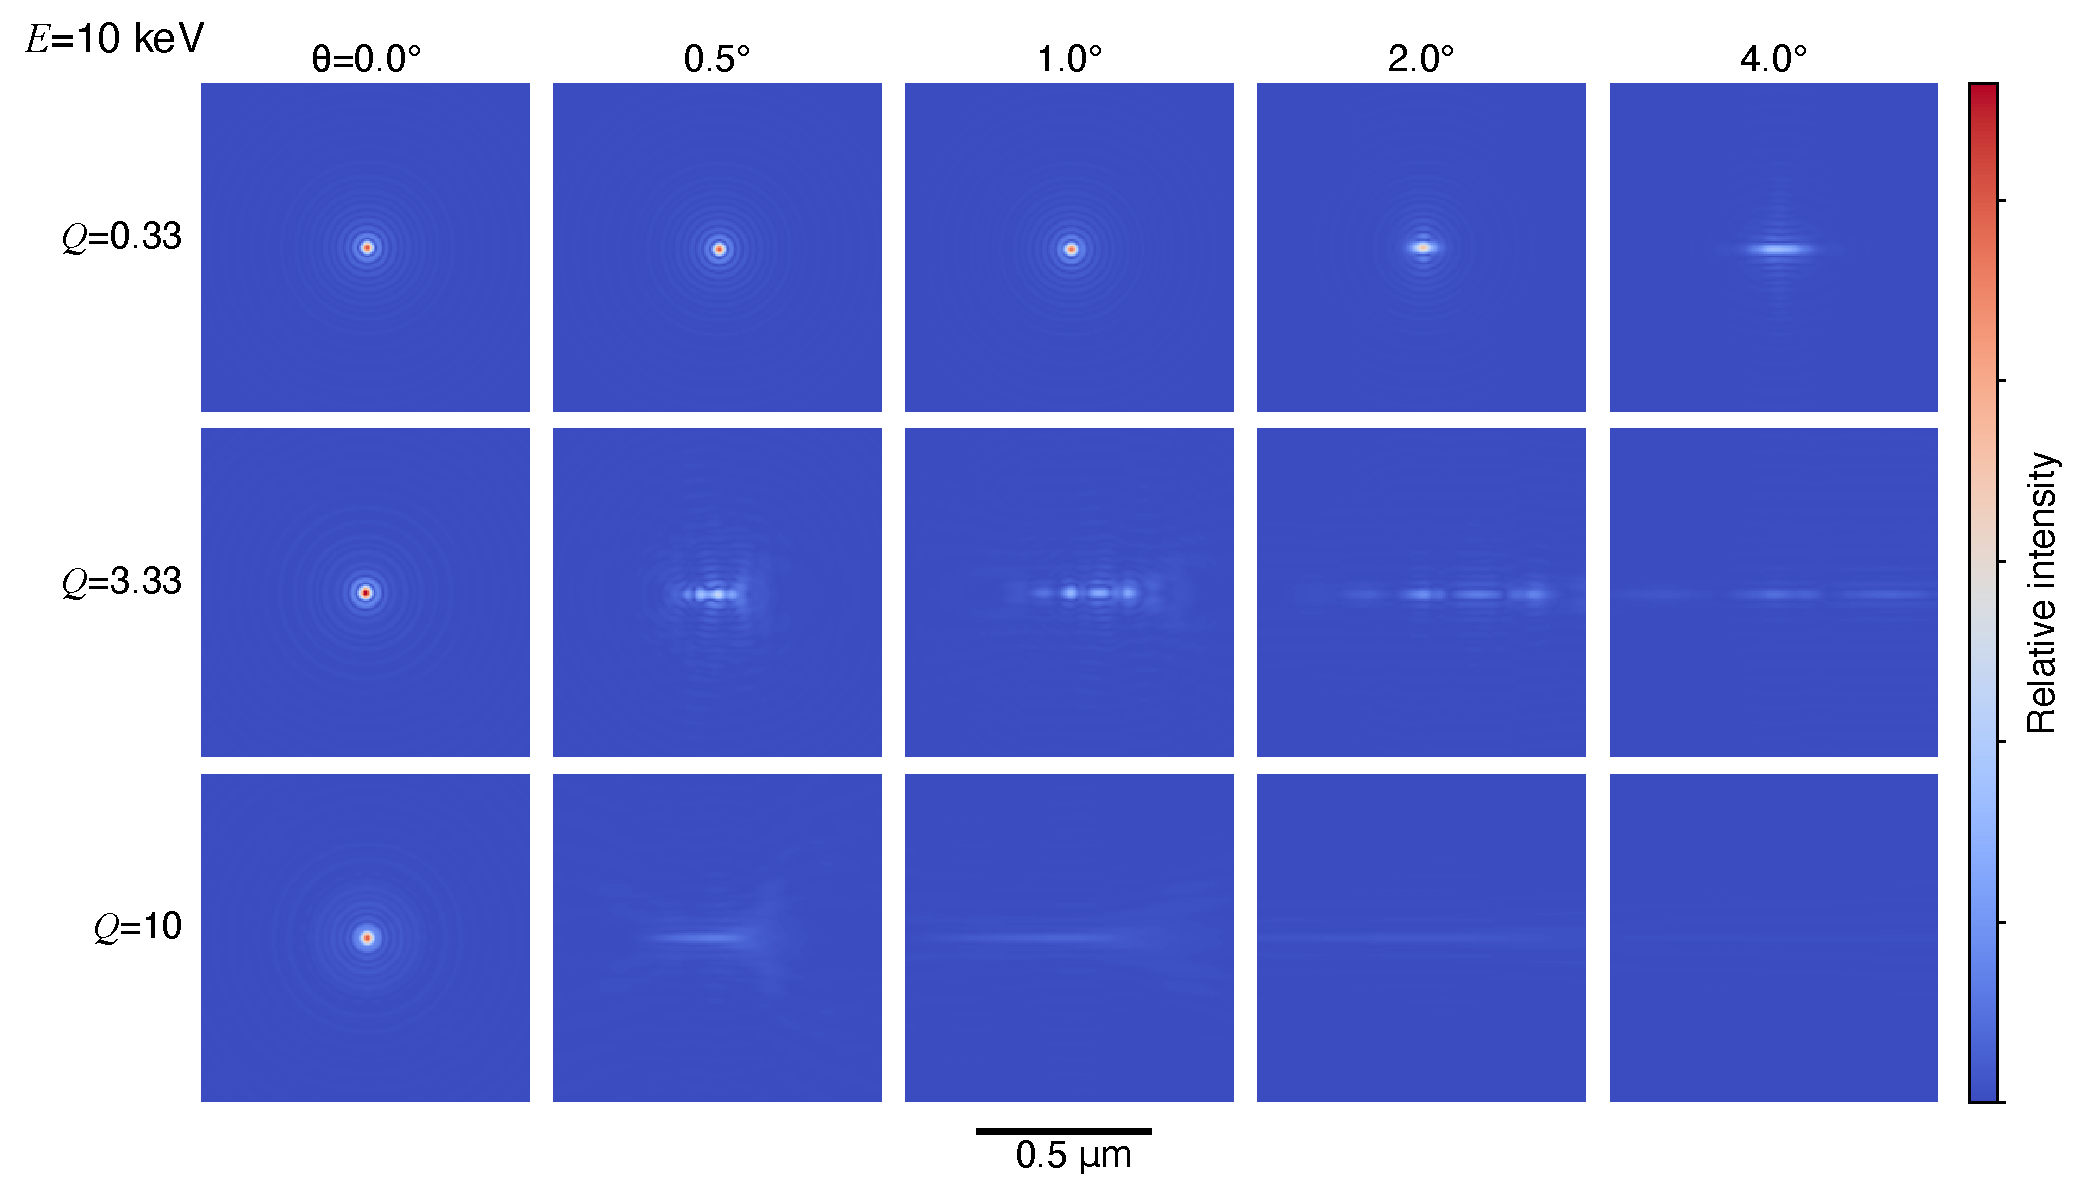
\includegraphics[scale=0.275]{foc_spot_ten}
				\caption{Partial fil}	
			\end{figure}
		\end{center}
	\end{itemize}
\end{frame}

\begin{frame}{soft x-ray}
	\begin{itemize}
		\item Limit agrees with analytic expectation.
		\begin{center}
			\begin{figure}
				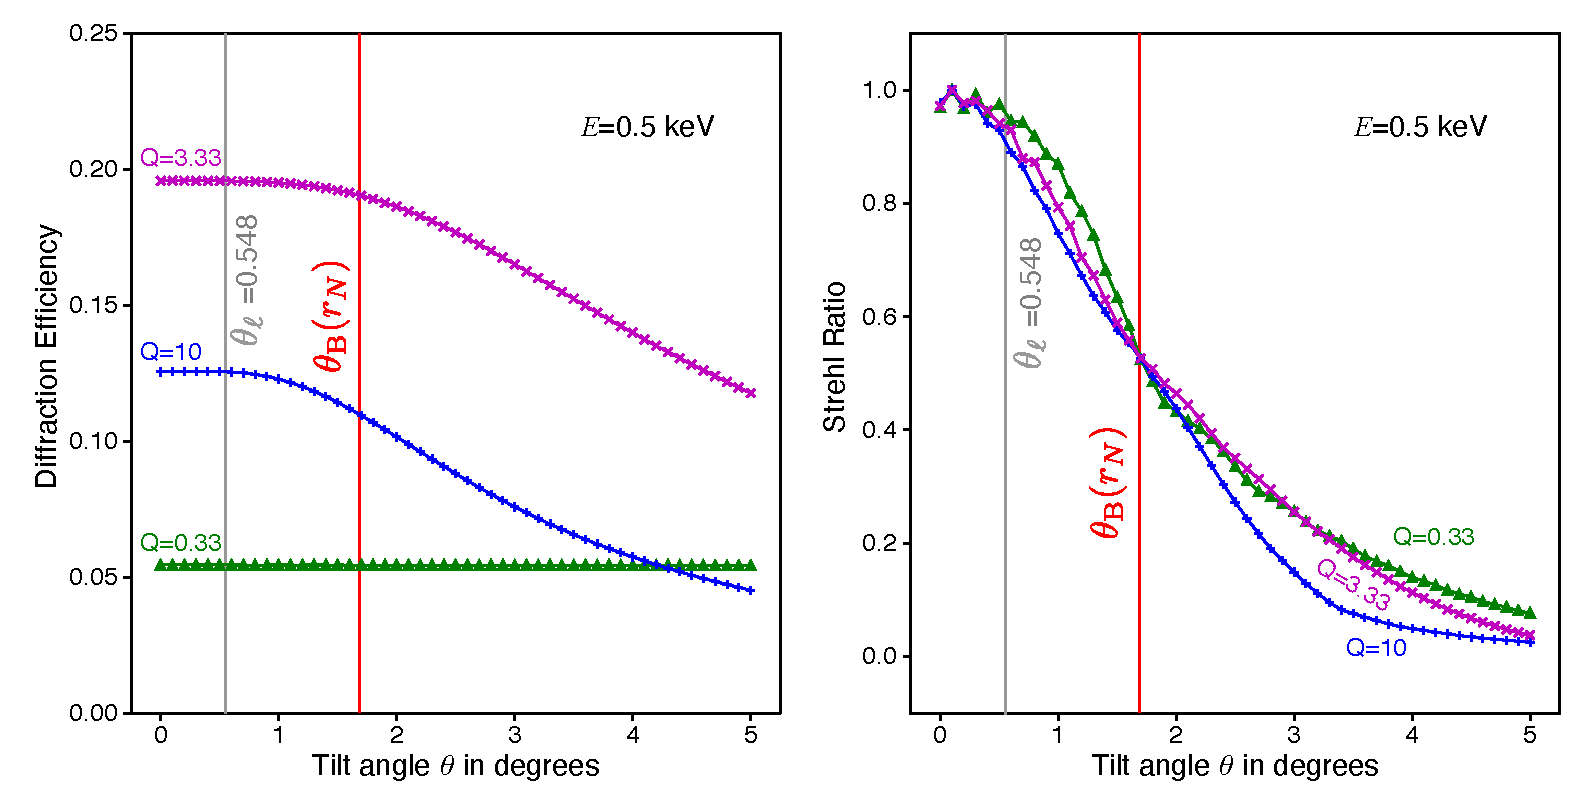
\includegraphics[scale=0.275]{tilt_plot_half}
				\caption{Partial fil}	
			\end{figure}
		\end{center}
	\end{itemize}
\end{frame}

\begin{frame}{hard x-ray}
	\begin{itemize}
		\item Limit agrees with analytic expectation.
		\begin{center}
			\begin{figure}
				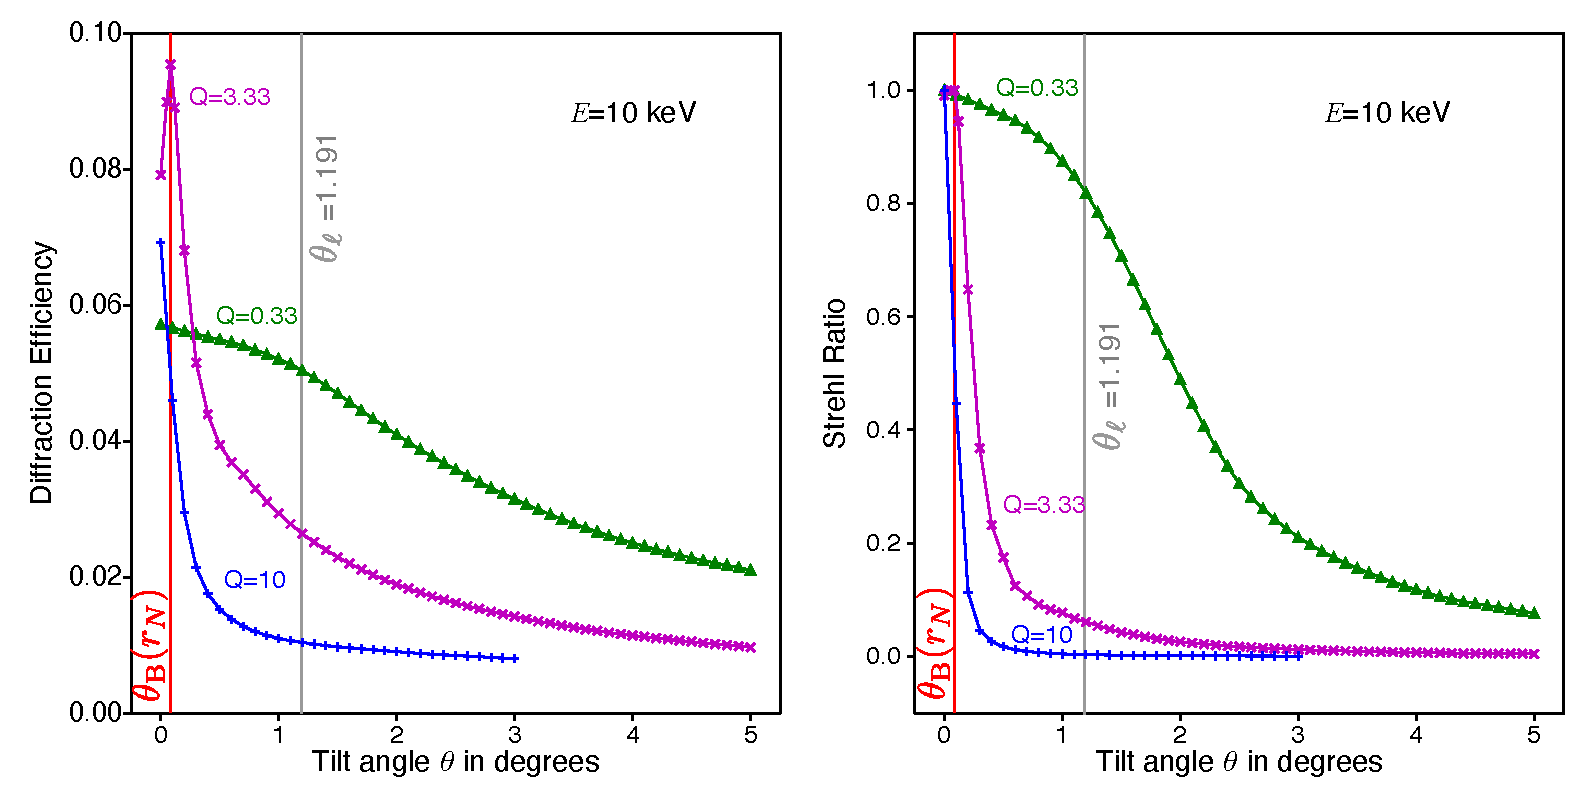
\includegraphics[scale=0.275]{tilt_plot_ten}
				\caption{Partial fil}	
			\end{figure}
		\end{center}
	\end{itemize}
\end{frame}



%\begin{comment}
% Placing a * after \section means it will not show in the
% outline or table of contents.

\begin{frame}{Acknowledgements}
  \begin{itemize}
  \item \alert{Kenan Li} SLAC
  \item \alert{Michael Wojcik} APS,ANL.
  \item \alert{NIMH} U01 MH109100
  \end{itemize}
\end{frame}

%\end{comment}

% All of the following is optional and typically not needed. 
%\appendix
\renewcommand*{\bibfont}{\scriptsize}
\begin{frame}[t, allowframebreaks]
\frametitle{References}
\bibliographystyle{dinat-etal}
\bibliography{xsd_coffee_talk}
\end{frame}

\end{document}

